\chapter{Конструкторский раздел}

\section{Функциональная модель и состав решения}

Граница разрабатываемого решения включает приём USB-пакетов, проверку данных, вычисление относительного смещения и передачу состояний кнопок. Отрисовка указателя остаётся за пределами модуля. Контекстная диаграмма IDEF0 приведена на рисунке~\ref{fig:idef0}. Её входы --- отчёты стилуса и события подключения; выходы --- перемещения, состояния кнопок и диагностика. Управление задаётся форматом отчёта, правилами преобразования и требованиями API ядра; механизмы представлены USB-подсистемой, модулем и подсистемой ввода.

\begin{figure}[H]
\centering
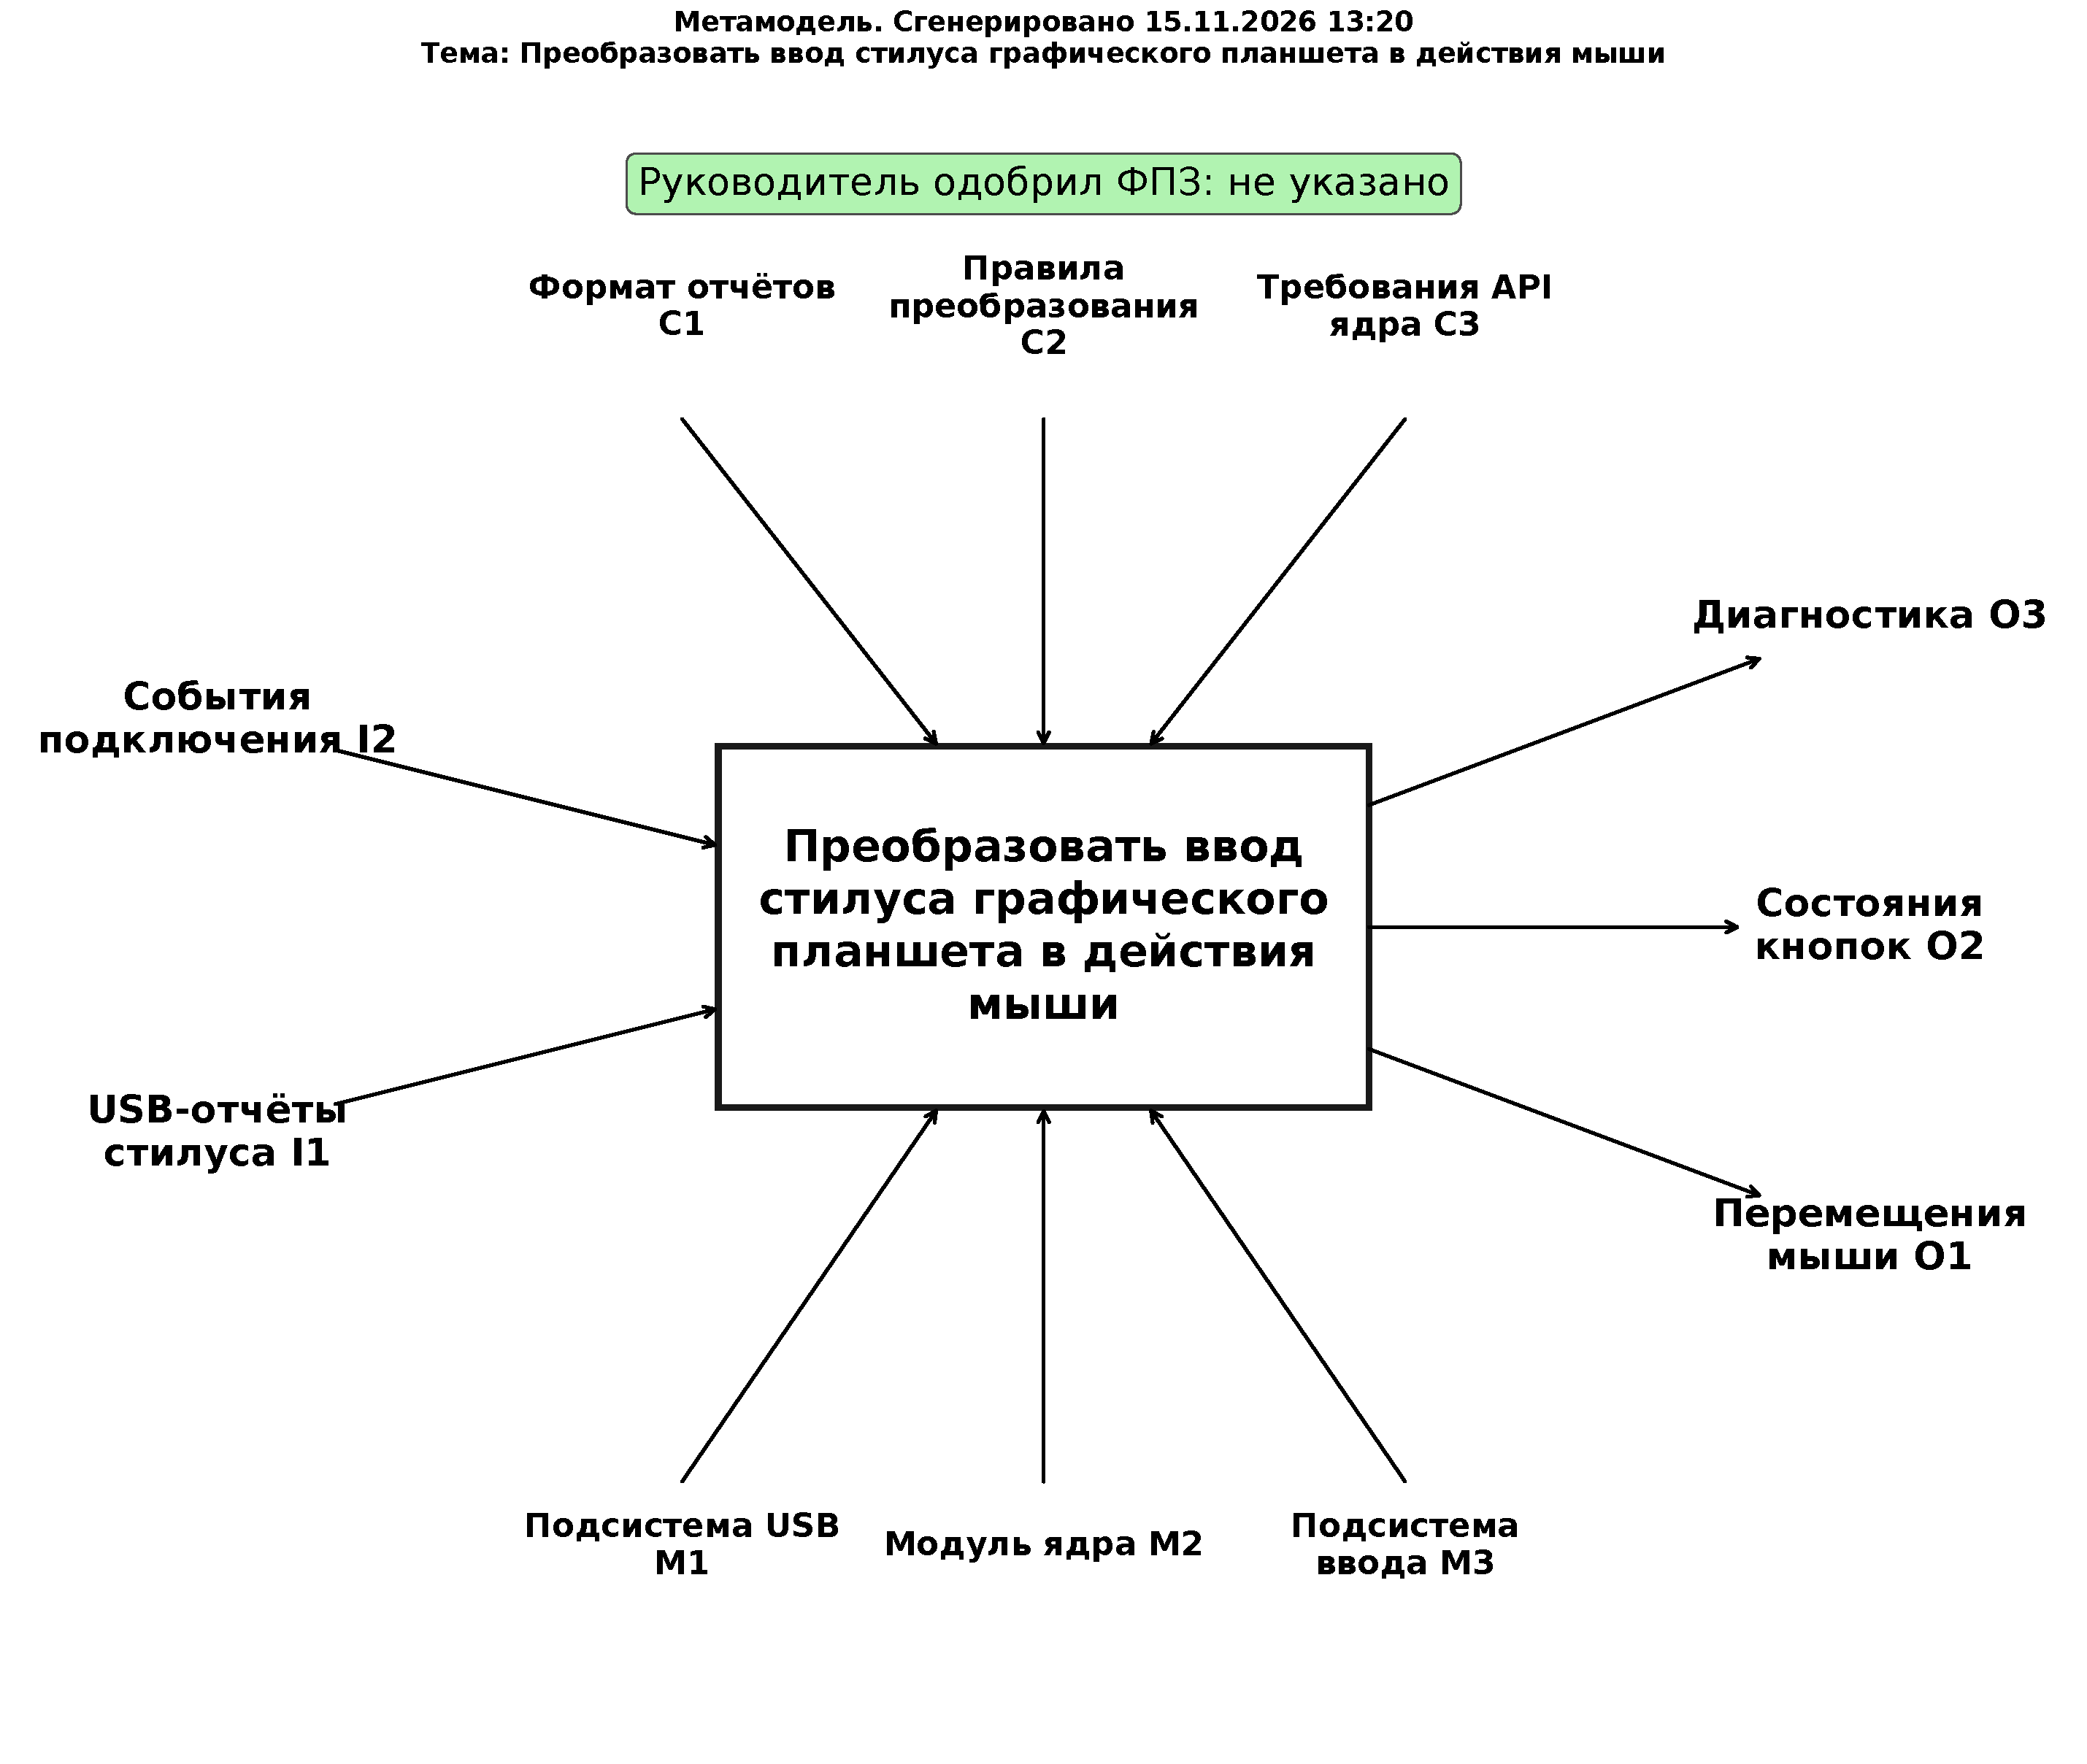
\includegraphics[width=\textwidth,height=0.55\textheight,keepaspectratio]{idef0/idef0_a0_diagram.pdf}
\caption{Контекстная диаграмма преобразования ввода стилуса}
\label{fig:idef0}
\end{figure}

Решение состоит из модуля ядра и административного средства управления привязками. Модуль принимает пакеты через URB и формирует устройство мыши; средство управления переключает выбранные USB-интерфейсы между штатным и разработанным драйверами. Оно не участвует в обработке движения. События передаются по цепочке «USB core --- драйвер --- Linux Input Subsystem --- пользовательское окружение»~\cite{kernelusb,kernelinput}.

Интерфейс пера используется для чтения данных. Интерфейс совместимости временно занимается без опроса и регистрации устройства ввода, чтобы исключить дублирование событий. Вспомогательные интерфейсы сохраняют штатную обработку. Подмена HID-дескриптора не применяется. Соответствие номеров интерфейсов их ролям определяется аппаратным профилем, исследуемым далее.

\section{Структуры данных и точки входа}

Каждому устройству пера соответствует собственный контекст \path{xppen_mouse}. Он связывает ресурсы и состояние преобразования, не допуская смешения отсчётов нескольких устройств. Назначение данных приведено в таблице~\ref{tab:design-data}.

\begin{table}[H]
\caption{Данные контекста устройства}
\label{tab:design-data}
\centering\small
\begin{tabular}{|p{0.28\textwidth}|p{0.63\textwidth}|}\hline
Данные & Назначение \\ \hline
USB-ресурсы & Удерживаемая ссылка на устройство, интерфейс, URB и канал передачи \\ \hline
Буфер и устройство ввода & Адрес памяти, DMA-адрес, размер буфера и \path{input_dev} \\ \hline
Состояние пера & Предыдущие координаты, остатки деления и признак начала отсчёта \\ \hline
Синхронизация & Спин-блокировка, разрешение отправки и работа восстановления \\ \hline
\end{tabular}
\end{table}

Структура \path{pen_state} хранит начало отсчёта и остатки масштабирования; \path{mouse_frame} --- приращения осей и состояния кнопок одного кадра. Признак \path{valid} отличает действительный отсчёт от начальных нулей памяти. Регистрация драйвера допускается при отсутствии планшета: обработка устройства начинается после сопоставления интерфейса и вызова \path{probe}.

В структуре \path{usb_driver} задаются подключение \path{xppen_probe}, отключение \path{xppen_disconnect}, приостановка \path{xppen_suspend}, возобновление \path{xppen_resume} и подготовка сброса \path{xppen_pre_reset}. После сброса применяется общий путь возобновления. Инициализация и завершение модуля соответственно регистрируют и удаляют сам драйвер.

\section{Алгоритмы работы}

Оригиналы схем подготовлены в каталоге \path{diagram} в формате GraphML. В рисунках~\ref{fig:probe-flow}--\ref{fig:binding-flow} временно используются согласованные PDF-заглушки; их содержимое заменяется экспортированными схемами при окончательной подготовке графической части.

\subsection{Подключение интерфейса пера}

Алгоритм \path{probe.graphml} проверяет назначение интерфейса. Для пера выбирается входная interrupt-конечная точка; её размер пакета и интервал берутся из дескриптора. Выделяются контекст, URB, DMA-буфер и устройство ввода с относительными осями и двумя кнопками. После регистрации включается Report Protocol и запускается приём. Ошибка на любом этапе приводит к освобождению уже полученных ресурсов; зарегистрированное устройство снимается с регистрации отдельно от ещё не зарегистрированного~\cite{kernelusb,kernelinput}.

\begin{figure}[H]
\centering
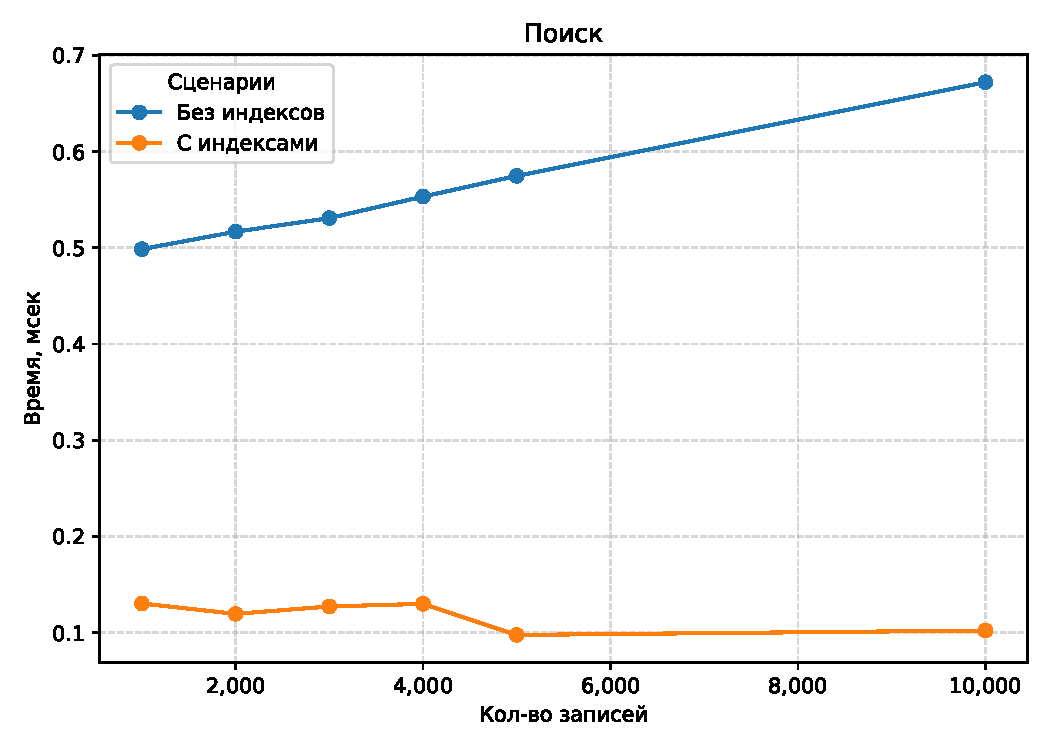
\includegraphics[width=0.72\textwidth,height=0.20\textheight,keepaspectratio]{pdf/Поиск.pdf}
\caption{Схема подключения интерфейса пера}
\label{fig:probe-flow}
\end{figure}

\subsection{Завершение USB-запроса}

Сначала проверяется разрешение приёма (\path{complete.graphml}). Успешно полученный пакет передаётся декодеру; допустимый результат публикуется через функции \path{input_report_rel()}, \path{input_report_key()} и \path{input_sync()}. Статусы отмены прекращают цикл, остановка конечной точки запускает восстановление. После прочих ошибок выполняются ограниченная по частоте диагностика и повторная отправка URB. Ошибка отправки снимает разрешение приёма и освобождает кнопки.

\begin{figure}[H]
\centering
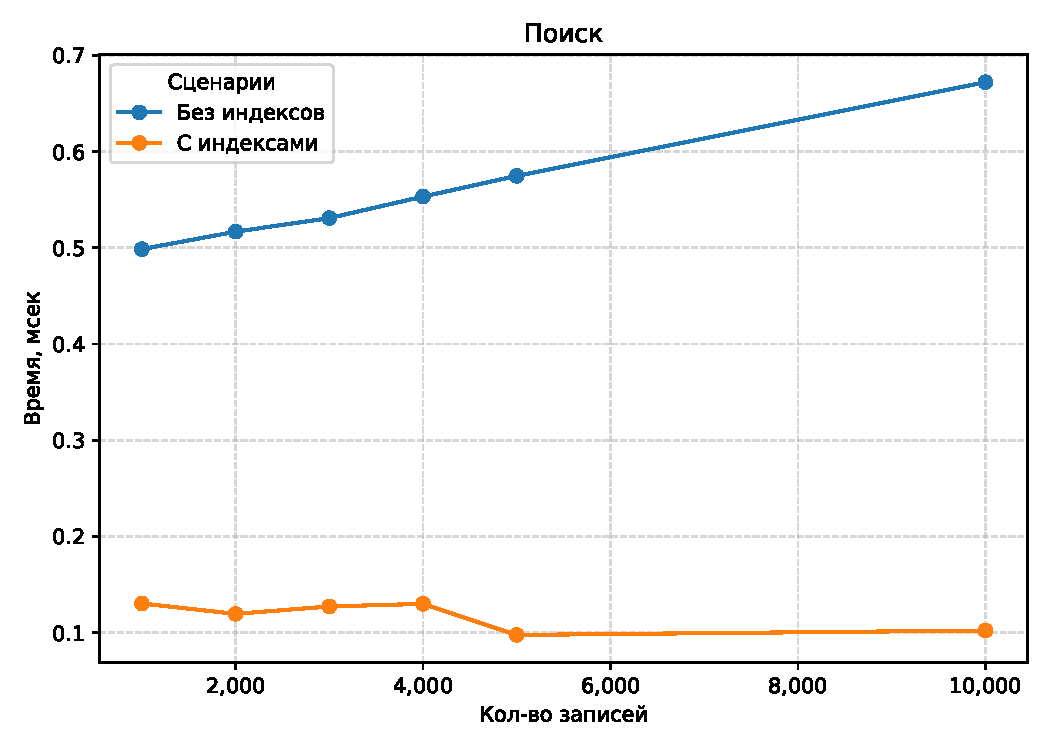
\includegraphics[width=0.72\textwidth,height=0.20\textheight,keepaspectratio]{pdf/Поиск.pdf}
\caption{Схема завершения USB-запроса}
\label{fig:complete-flow}
\end{figure}

\subsection{Преобразование координат и кнопок}

Алгоритм \path{decode.graphml} проверяет формат до изменения состояния. Пусть $x_k$ --- текущая координата, $d>0$ --- делитель, $r^x_{k-1}$ --- сохранённый остаток. Для оси $x$ применяется
\begin{equation}
 s^x_k=x_k-x_{k-1}+r^x_{k-1},\quad
 \Delta x_k=\operatorname{trunc}(s^x_k/d),\quad
 r^x_k=s^x_k-d\Delta x_k.
 \label{eq:relative-x}
\end{equation}
Операция $\operatorname{trunc}$ означает усечение к нулю. Это правило знакового деления C99~\cite{c99}; для оси $y$ расчёт аналогичен. Сохранение остатка учитывает малые смещения и компенсирует противоположные движения. Ошибка накопленного масштабирования при неизменном начале отсчёта меньше одной выходной единицы.

Первый отсчёт только запоминается. Касание задаёт удержание ЛКМ, основная боковая кнопка --- ПКМ. При выходе пера обе кнопки освобождаются, начало отсчёта и остатки сбрасываются. Поэтому возвращение пера в другой точке не вызывает скачка. Отчёт выхода обрабатывается до проверки координат, поскольку они могут быть неопределёнными.

\begin{figure}[H]
\centering
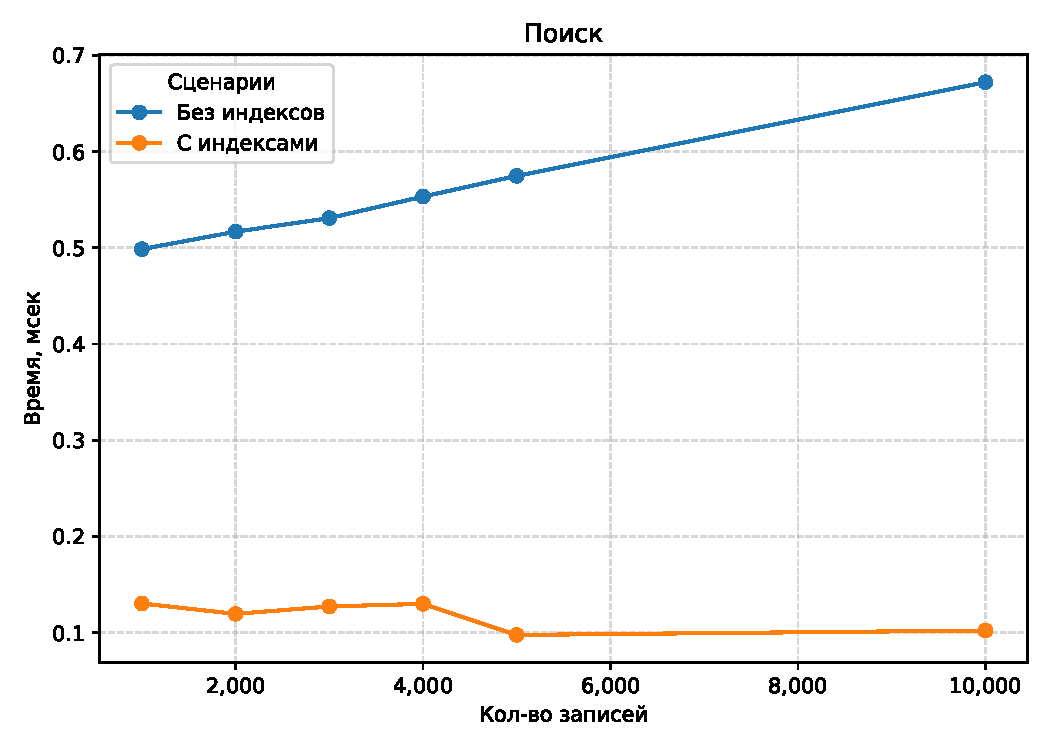
\includegraphics[width=0.72\textwidth,height=0.20\textheight,keepaspectratio]{pdf/Поиск.pdf}
\caption{Схема преобразования отчёта пера}
\label{fig:decode-flow}
\end{figure}

\subsection{Остановка приёма}

Алгоритм \path{stop.graphml} под спин-блокировкой запрещает повторную отправку. Та же блокировка защищает проверку разрешения и отправку из completion callback, устраняя гонку с отключением. Затем вне блокировки выполняются \path{usb_kill_urb()} и \path{cancel_work_sync()}. После ожидания освобождаются кнопки; при отключении дополнительно отменяется регистрация устройства и возвращаются ресурсы. Освобождение памяти до завершения обработчиков недопустимо~\cite{kernelusb}.

\begin{figure}[H]
\centering
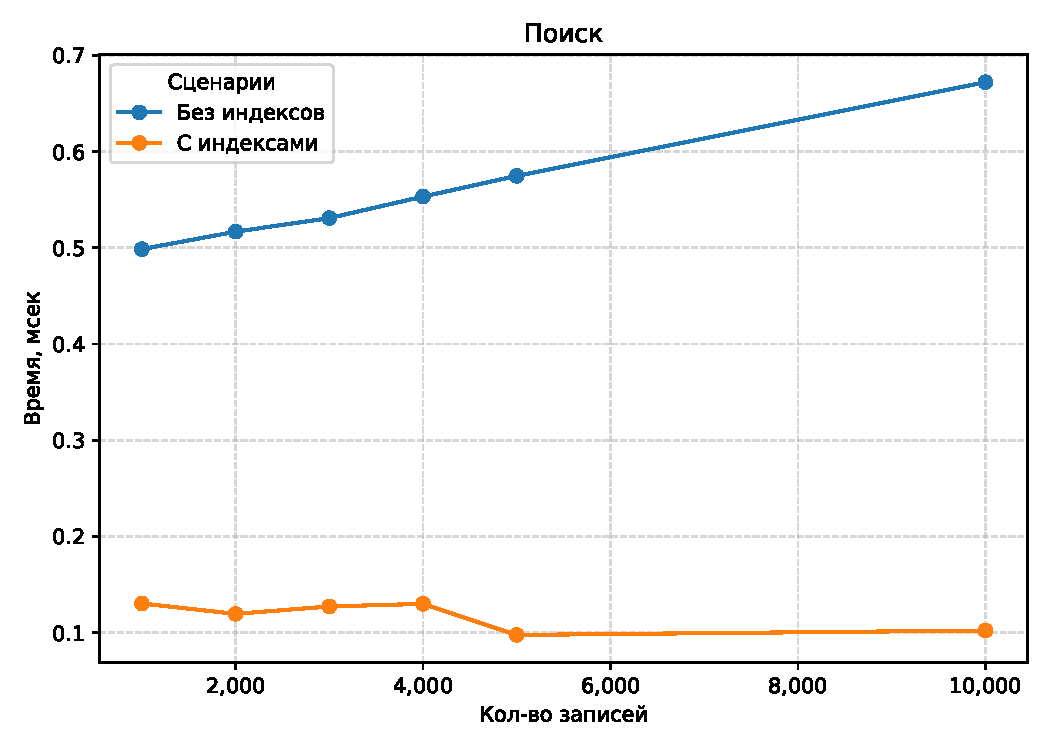
\includegraphics[width=0.72\textwidth,height=0.20\textheight,keepaspectratio]{pdf/Поиск.pdf}
\caption{Схема остановки приёма}
\label{fig:stop-flow}
\end{figure}

\subsection{Восстановление конечной точки}

Алгоритм \path{recovery.graphml} выполняется в рабочей очереди, поскольку \path{usb_clear_halt()} допускает ожидание. После очистки под блокировкой повторно проверяется разрешение приёма. Если остановка уже началась, обмен не возобновляется. При сохранённом разрешении запрос отправляется снова; ошибка восстановления прекращает приём и освобождает кнопки. Путь отключения ожидает рабочую функцию, сохраняя действительность её контекста.

\begin{figure}[H]
\centering
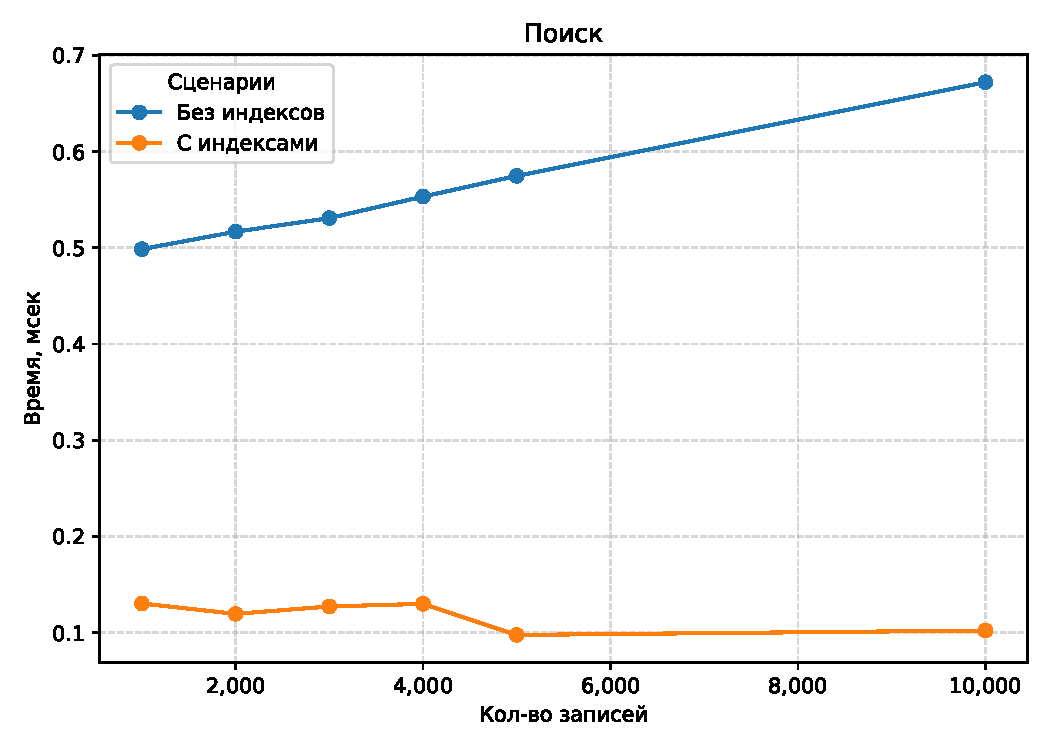
\includegraphics[width=0.72\textwidth,height=0.20\textheight,keepaspectratio]{pdf/Поиск.pdf}
\caption{Схема восстановления конечной точки}
\label{fig:recovery-flow}
\end{figure}

\subsection{Управление привязками}

Алгоритм \path{binding.graphml} отбирает поддерживаемые интерфейсы через sysfs и сохраняет предыдущие привязки до изменения. Сначала переключается интерфейс совместимости, затем интерфейс пера. При ошибке уже затронутые интерфейсы восстанавливаются в обратном порядке. Записи о неудачном восстановлении сохраняются для повторной команды. Файловая блокировка сериализует административные операции; перед восстановлением заново проверяются идентификаторы устройства, а не только старое имя пути.

\begin{figure}[H]
\centering
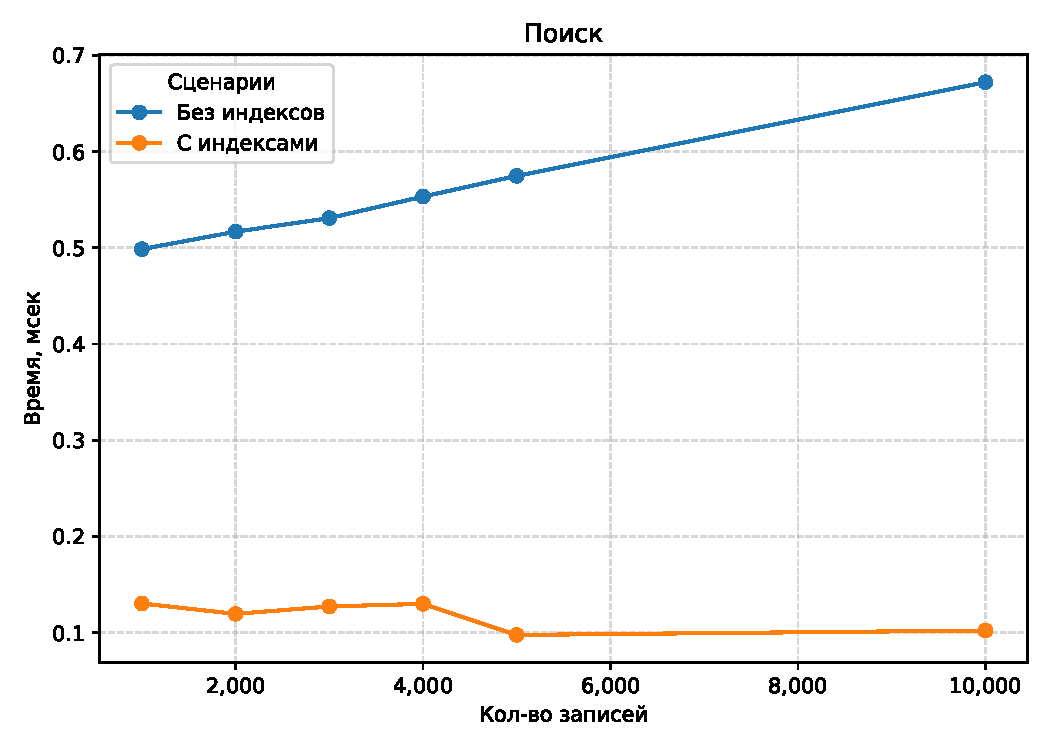
\includegraphics[width=0.72\textwidth,height=0.20\textheight,keepaspectratio]{pdf/Поиск.pdf}
\caption{Схема переключения привязок}
\label{fig:binding-flow}
\end{figure}

Определены структура решения, точки входа и алгоритмы обработки. Масштабирование сохраняет остатки, а потеря пера сбрасывает начало отсчёта. Согласованный порядок остановки запрещает новые запросы до ожидания обработчиков и освобождения памяти.

\clearpage
